
\subsection{Term unfolding for homogeneous inputs}
\label{sec:homo-unfold}


---------------------------------------------------------------------------------------------------------------------------------------------------------
List of functions I need for this proof:
\begin{align*}
\ranked{\Gamma_1\otimes\Gamma_2 \to \reduce 1 \Gamma_i}\\
\ranked{\Sigma\to \reduce 2 (\Sigma\otimes \Sigma)}\\
\ranked{\reduce k \Sigma \otimes \reduce k \Gamma \to \reduce k (\Sigma\otimes \Gamma)}\\
\ranked{\reduce k \Sigma \to \reduce {k+l} \Sigma }\\
\ranked{\reduce k\Sigma \to \reduce {k-l} {(\Sigma\cdot(0+1))}}\\
\ranked{\reduce k (\Gamma\otimes \Sigma) \to \reduce k (\reduce k \Gamma \otimes \Sigma)}\\
\ranked{\Gamma \leftrightarrow \Gamma\cdot 1}\\
\ranked{\reduce k \Gamma\cdot(\Sigma_1+\Sigma_2)\to \reduce k(\reduce k \Gamma\cdot(\Sigma_1+\Sigma_2))}
\end{align*}
I need operations transforming tensors and shallow terms into terms and vice et versa.
I need associativity of $\cdot$ and $\otimes$.
I need also to derive this:
\begin{align*}
\ranked{\reduce k \tmonad\Sigma\cdot\Gamma\to \reduce k \tmonad\Sigma}
\end{align*}
To derive t, I will need the following derivable function
\begin{align*}
\ranked{\reduce k \Sigma\cdot \Gamma\to \reduce k (\Sigma\cdot \Gamma)}
\end{align*}
We need also a "partial shallow unfold"
\begin{align*}
\ranked{\reduce k (\Sigma\cdot (1+\Gamma^k))\to \reduce k (\Sigma\cdot(1+\Gamma))}
\end{align*}

---------------------------------------------------------------------------------------------------------------------------------------------------------
\bigskip

For a monotone function 
\begin{align*}
\alpha: \set{1,\ldots,k} \to \set{1,\ldots,k}
\end{align*}
we say that a term $ t \in \tmonad \mati k \rSigma$ is $\alpha$-homogeneous if all internal branches have twist $\alpha$. This section is devoted to proving the following lemma. 

\begin{lemma}\label{lem:homo-twist}
    Let $k \in \set{1,2,\ldots}$ and let $\alpha : \set{1,\ldots,k} \to \set{1,\ldots,k}$ be a monotone function. There is a derivable operation 
    \begin{align*}
        \ranked{f : \tmonad \mati k \rSigma \to \mati k {(\tmonad \Sigma)} }
        \end{align*}      
which coincides with term unfolding for all inputs which are $\alpha$-homogeneous.
\end{lemma}

In order to prove lemma~\ref{lem:homo-twist}, we need to show that a very particular form of unfolding, which we call \emph{the unfolding of external twists}, is derivable. This function, which is of type 
\begin{align*}
\ranked{\tmonad \mati k \Sigma \to \reduce k \tmonad \mati k \Sigma}
\end{align*}
"untwists" the external twists  as illustrated by the following figure where the external twists have been coloured in red. 
\begin{center}
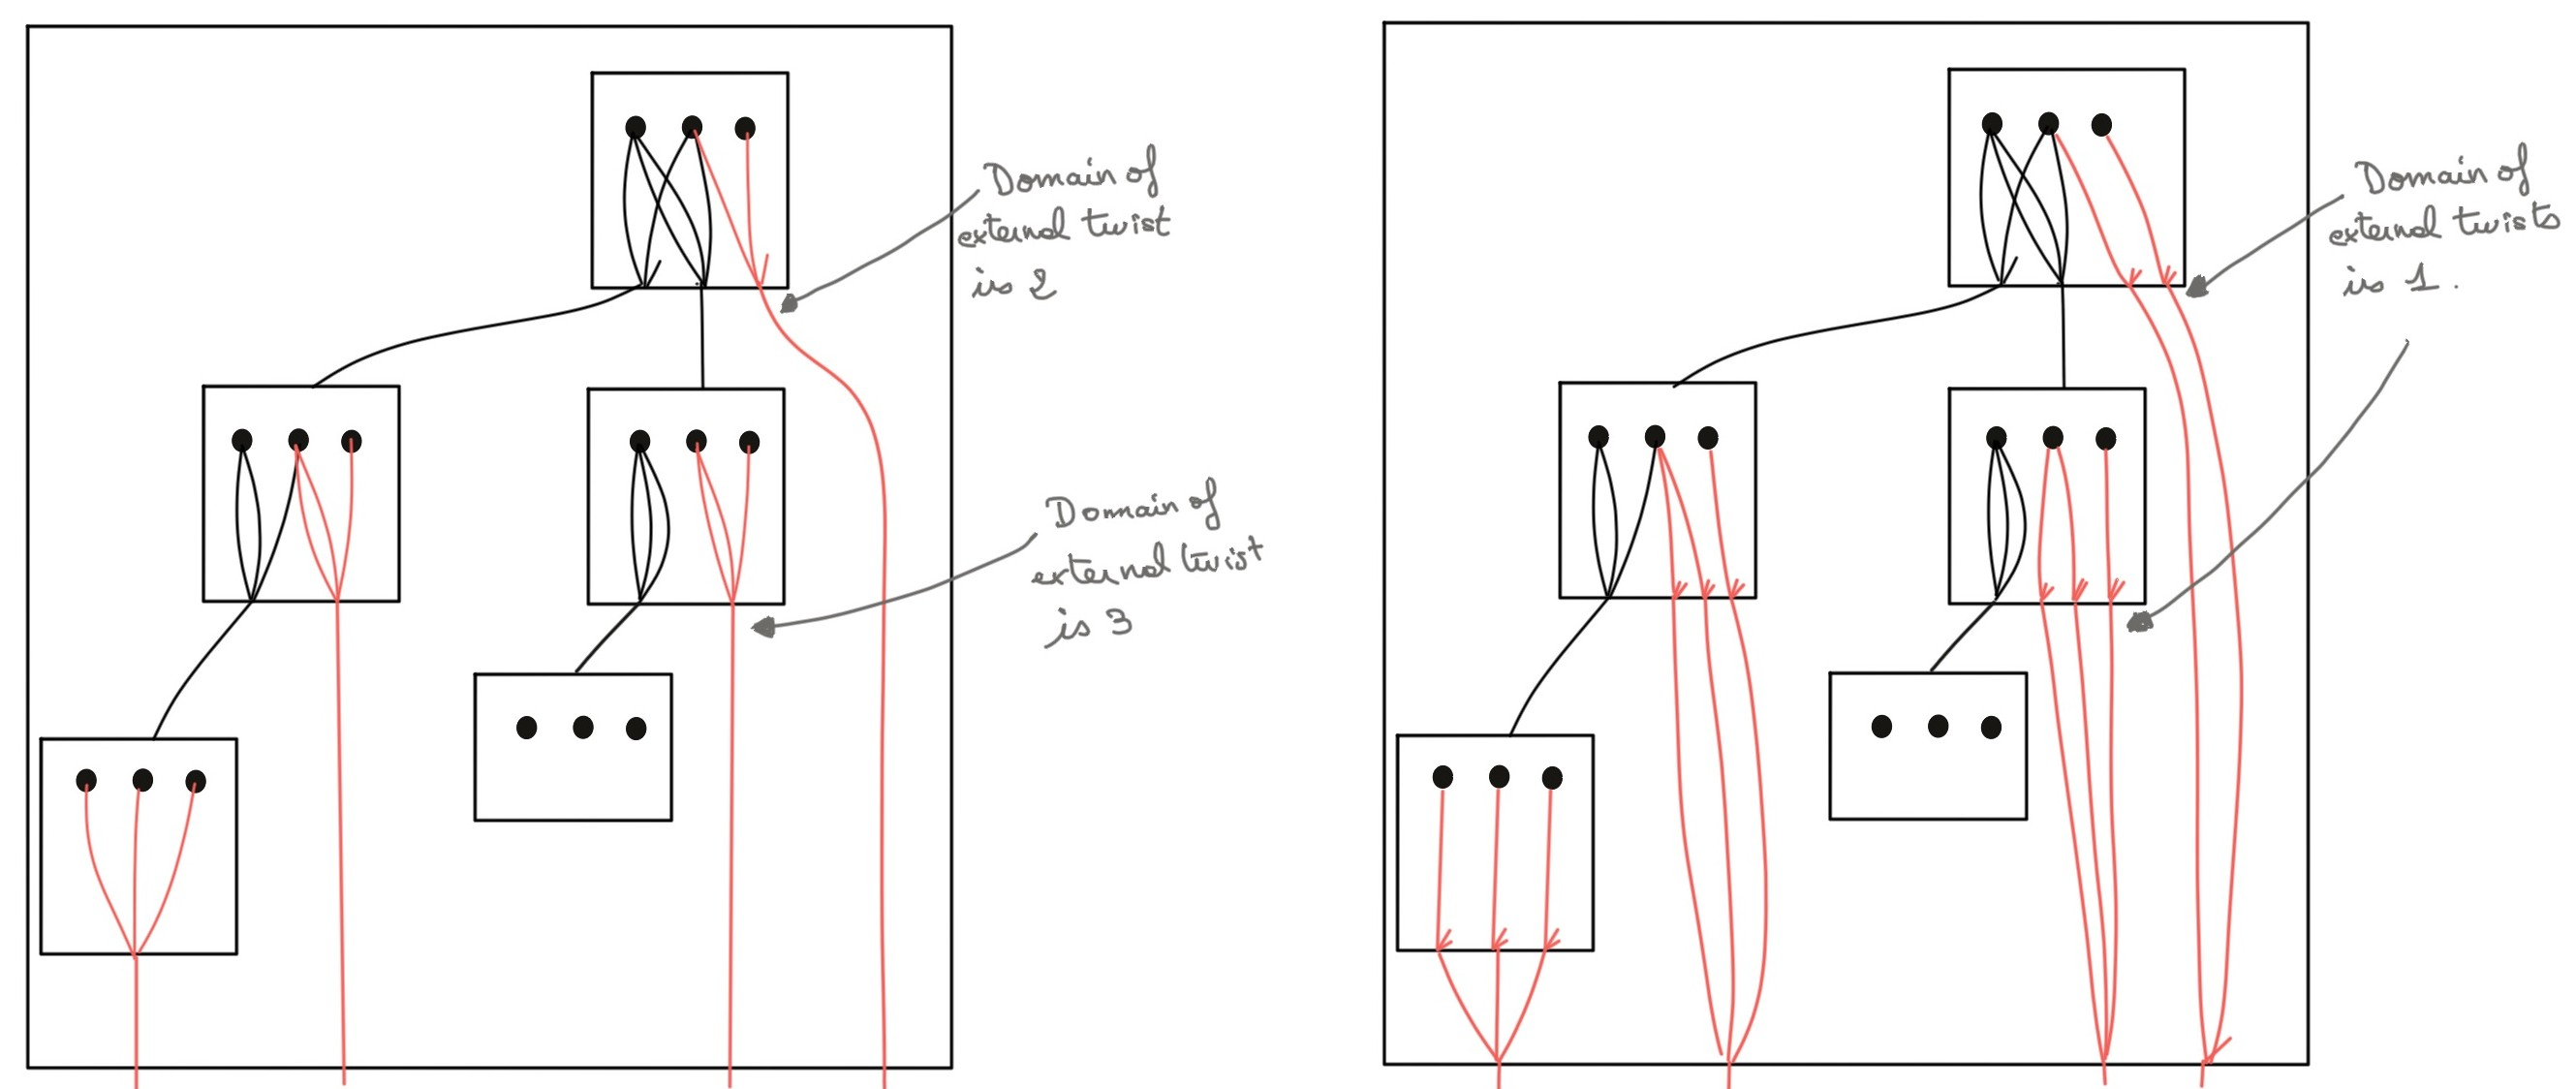
\includegraphics[scale=.15]{MyPicExternalTwists.jpg}
\end{center}
The main feature of this function, which will be very useful later, is that the external twists of the output term (more precisely the term of $\ranked{\tmonad \mati k \Sigma}$ underlying the output) have $1$ as domain.  

If $u$ is an element of $\ranked{\reduce k \Sigma}$, let us denote by $\overline{u}$ the term of $\ranked{\Sigma}$ underlying it.
\begin{lemma}\label{lem:unfold-external-twist}
There is a derivable function
\begin{align*}
\ranked{f:\tmonad \mati k \Sigma \to \reduce k \tmonad \mati k \Sigma}
\end{align*}
satisfying the follwoing conditions:
\begin{itemize}
\item The function $f$ preserves the unfolding. More precisely:
\begin{align*}
\ranked{\reduce k(\mathsf{Unfold})\circ f}=\ranked{\mathsf{Unfold}}
\end{align*} 
\item It preserves $\alpha$-homogenuity. That is, if $t\in\ranked{\tmonad\mati k \rSigma}$ is $\alpha$-homogeneous, then so is $\overline{f(t)}$.
\item  For every term $t\in \ranked{\tmonad\mati k \rSigma}$, the domain of the external twists of $\overline{f(t)}$ is 1.
\end{itemize}
We call $f$ an external unfold function.
\end{lemma}
\begin{proof}
Some combinator is missing to do this.
\end{proof}
\begin{proof}[Proof of Lemma~\ref{lem:homo-twist}]
We proceed by induction on $k$. When $k=1$, the unfolding coincides with the basic function 
\begin{align*}
\ranked{\distrtf : \tmonad \reduce 1 \Sigma \to {\reduce 1 \tmonad \Sigma}}
\end{align*}
Let us treat the inductive case. For that, we indroduce a tool that will be useful to analyse the function $\alpha$. For a function $$\alpha: \set{1,\ldots,k} \to \set{1,\ldots,k}$$ define  \emph{its graph} as the directed graph whose set of vertices is $\set{1,\ldots,k}$, and which contains an edge $i\rightarrow j$ if $\alpha(i)=j$. Note that the out-degree of the nodes is $1.$

\medskip
In the proof of the inductive case, we distinghuish two cases. The first is when the graph of $\alpha$ is not weakly connected. In this case, by monotonicity of $\alpha$, we can find $m\in \set{1,k-1}$ such that $\alpha(\set{1,m})\subseteq\set{1,m}$ and $\alpha(\set{m+1,k})\subseteq\set{m+1,k}$. The idea is then to create two copies of the original tree: in the first one we keep only the first $m$ elements of the tensor product of each node, and in the second one we keep the last $k-m$ copies. Then we unfold these terms by applying the induction hypothesis, and  finally we gather them to obtain the  unfolding of the original term. 

\smallskip
To implement these ideas, we start by unfolding the external twists, using the function from Lemma~\ref{lem:unfold-external-twist}. This way, the domain of every external twist has size at most one,  hence it cannot be shared by the two disconnected components of the domain of $\alpha$.
Then, we duplicate the input term using the basic function 
\begin{align*}
\ranked{\tmonad \mati k \Sigma\to \reduce 2 (\tmonad \mati k \Sigma\otimes \tmonad \mati k \Sigma)}
\end{align*}
To the first copy, we apply the function  
\begin{align*}
\ranked{f_1:\tmonad \mati k \Sigma \to \mati m {(\tmonad \Sigma)}}
\end{align*}
which keeps only the first $m$ elements of the tensor product, then applies the induction hypothesis to the obtained term. The function $f_1$ can be derived as follows. First, we consider the function which keeps only the first $m$ components of the tensor, obtained as the composition of the following tree functions:
\begin{align*}
\begin{prooftree}
\Hypo{\overbrace{\ranked{\mati k \Sigma \to \reduce k \reduce 1 \Sigma^m}}^{\substack{\text{Lift the projection on the first}\\\text{$m$ elements of the tensor to $\reduce k$}}}}
\Hypo{\overbrace{\ranked{\reduce k \reduce 1 \Sigma^m \to \reduce k \Sigma^m}}^{\substack{\text{Merge the folds $\reduce k$ and $\reduce 1$}}}}
\Hypo{\overbrace{\ranked{\reduce k \Sigma^m \to \mati m {(\Sigma\cdot (1+0))}}}^{\substack{\text{Adjust the degree of the fold}\\\text{to get a matrix power}}}}
\Infer{3}[]{\ranked{\mati k \Sigma \to \mati m {(\Sigma\cdot (1+0))}}}
\end{prooftree}
\end{align*}
We lif this function to terms, then we compose it with the following unfolding function, given by the induction hypothesis
\begin{align*}
\ranked{\tmonad \mati m {(\Sigma\cdot (1+0))} \to \mati m {(\tmonad (\Sigma\cdot (1+0)))}}
\end{align*}
Since $\rSigma$ contains a nullary element, we can embed the terms of  $\ranked{\tmonad (\Sigma\cdot (1+0))}$ into those of $\ranked{\tmonad \Sigma}$, obtaining finally the function $f_1$.

Similarly, we can derive the function
\begin{align*}
\ranked{f_2:\tmonad \mati k \Sigma \to \mati {k-m} {(\tmonad \Sigma)}}
\end{align*}
which keeps only the last $k-m$ elements of the tensor product, then applies the induction hypothesis to the obtained term.

When we apply $f_1$ and $f_2$ to the two copies of the original term, we get a term of type 
\begin{align*}
\ranked{ \reduce 2 (\mati m {(\tmonad \Sigma)}\otimes  \mati {k-m} {(\tmonad\Sigma)})}
\end{align*}
Now, we need to get the fold outsid the tensor product. For that, we lift both $\ranked{\mati m {(\tmonad \Sigma)}}$ and $\ranked{\mati {k-m} {(\tmonad \Sigma)}}$ to $\ranked{\reduce k (\tmonad \Sigma)^m}$ and $\ranked{\reduce k (\tmonad \Sigma)^{k-m}}$ respectively. Then we commute the fold with the tensor product using the following basic function:
\begin{align*}
\ranked{\reduce k (\tmonad \Sigma)^m\otimes\reduce k (\tmonad \Sigma)^{k-m}\to \reduce k (\tmonad \Sigma)^k}
\end{align*}
Then we merge the two  folds $\reduce 2$ and $\reduce k$ into $\reduce {2k}$. After these operations, we get the desired term, but not with the desired type (the type we get is $\ranked{\reduce {2k} (\tmonad\Sigma)^k}$. To get the right type which is $\ranked{\mati k {(\tmonad\Sigma)}}$, we apply the following function wich reducs the degree of the fold
\begin{align*}
\ranked{\reduce {2k} (\tmonad \Sigma)^k \to \reduce {k} (\tmonad \Sigma\cdot(0+1))^k}
 \end{align*}
then we embed the terms of $\ranked{\tmonad \Sigma\cdot(0+1)}$ into $\ranked{\tmonad \Sigma}$ using, as we did earlier, the fact that $\rSigma$ contains a nullary element, then getting the type $\ranked{\mati k {(\tmonad\Sigma)}}$.

\medskip
Now consider the case where the graph of $\alpha$ is weakly connected. By monotonicity, we can show that either
\begin{align*}
\alpha^{-1}(1)=\emptyset\qquad\text{ or }\qquad\alpha^{-1}(k)=\emptyset
\end{align*}
By symetry, we suppose wlog that $\alpha^{-1}(k)=\emptyset$. We suppose also that $\alpha(k)=k-1$, the general case can be treated in a similar way.
First of all, we apply the function given by lemma~\ref{lem:unfold-external-twist} to unfold the external twists.  Then we proceed in three steps. 
\begin{enumerate}
\item First, we apply the function
\begin{align*}
\ranked{\tmonad \mati k \Sigma \to \reduce k \tmonad(\reduce k\Sigma^{k-1}\otimes \Sigma)}
\end{align*} 
which isolates the last component of the tensor product. We illustrate the effect of the function $f$ by the following example, where $k=3$
\begin{center}
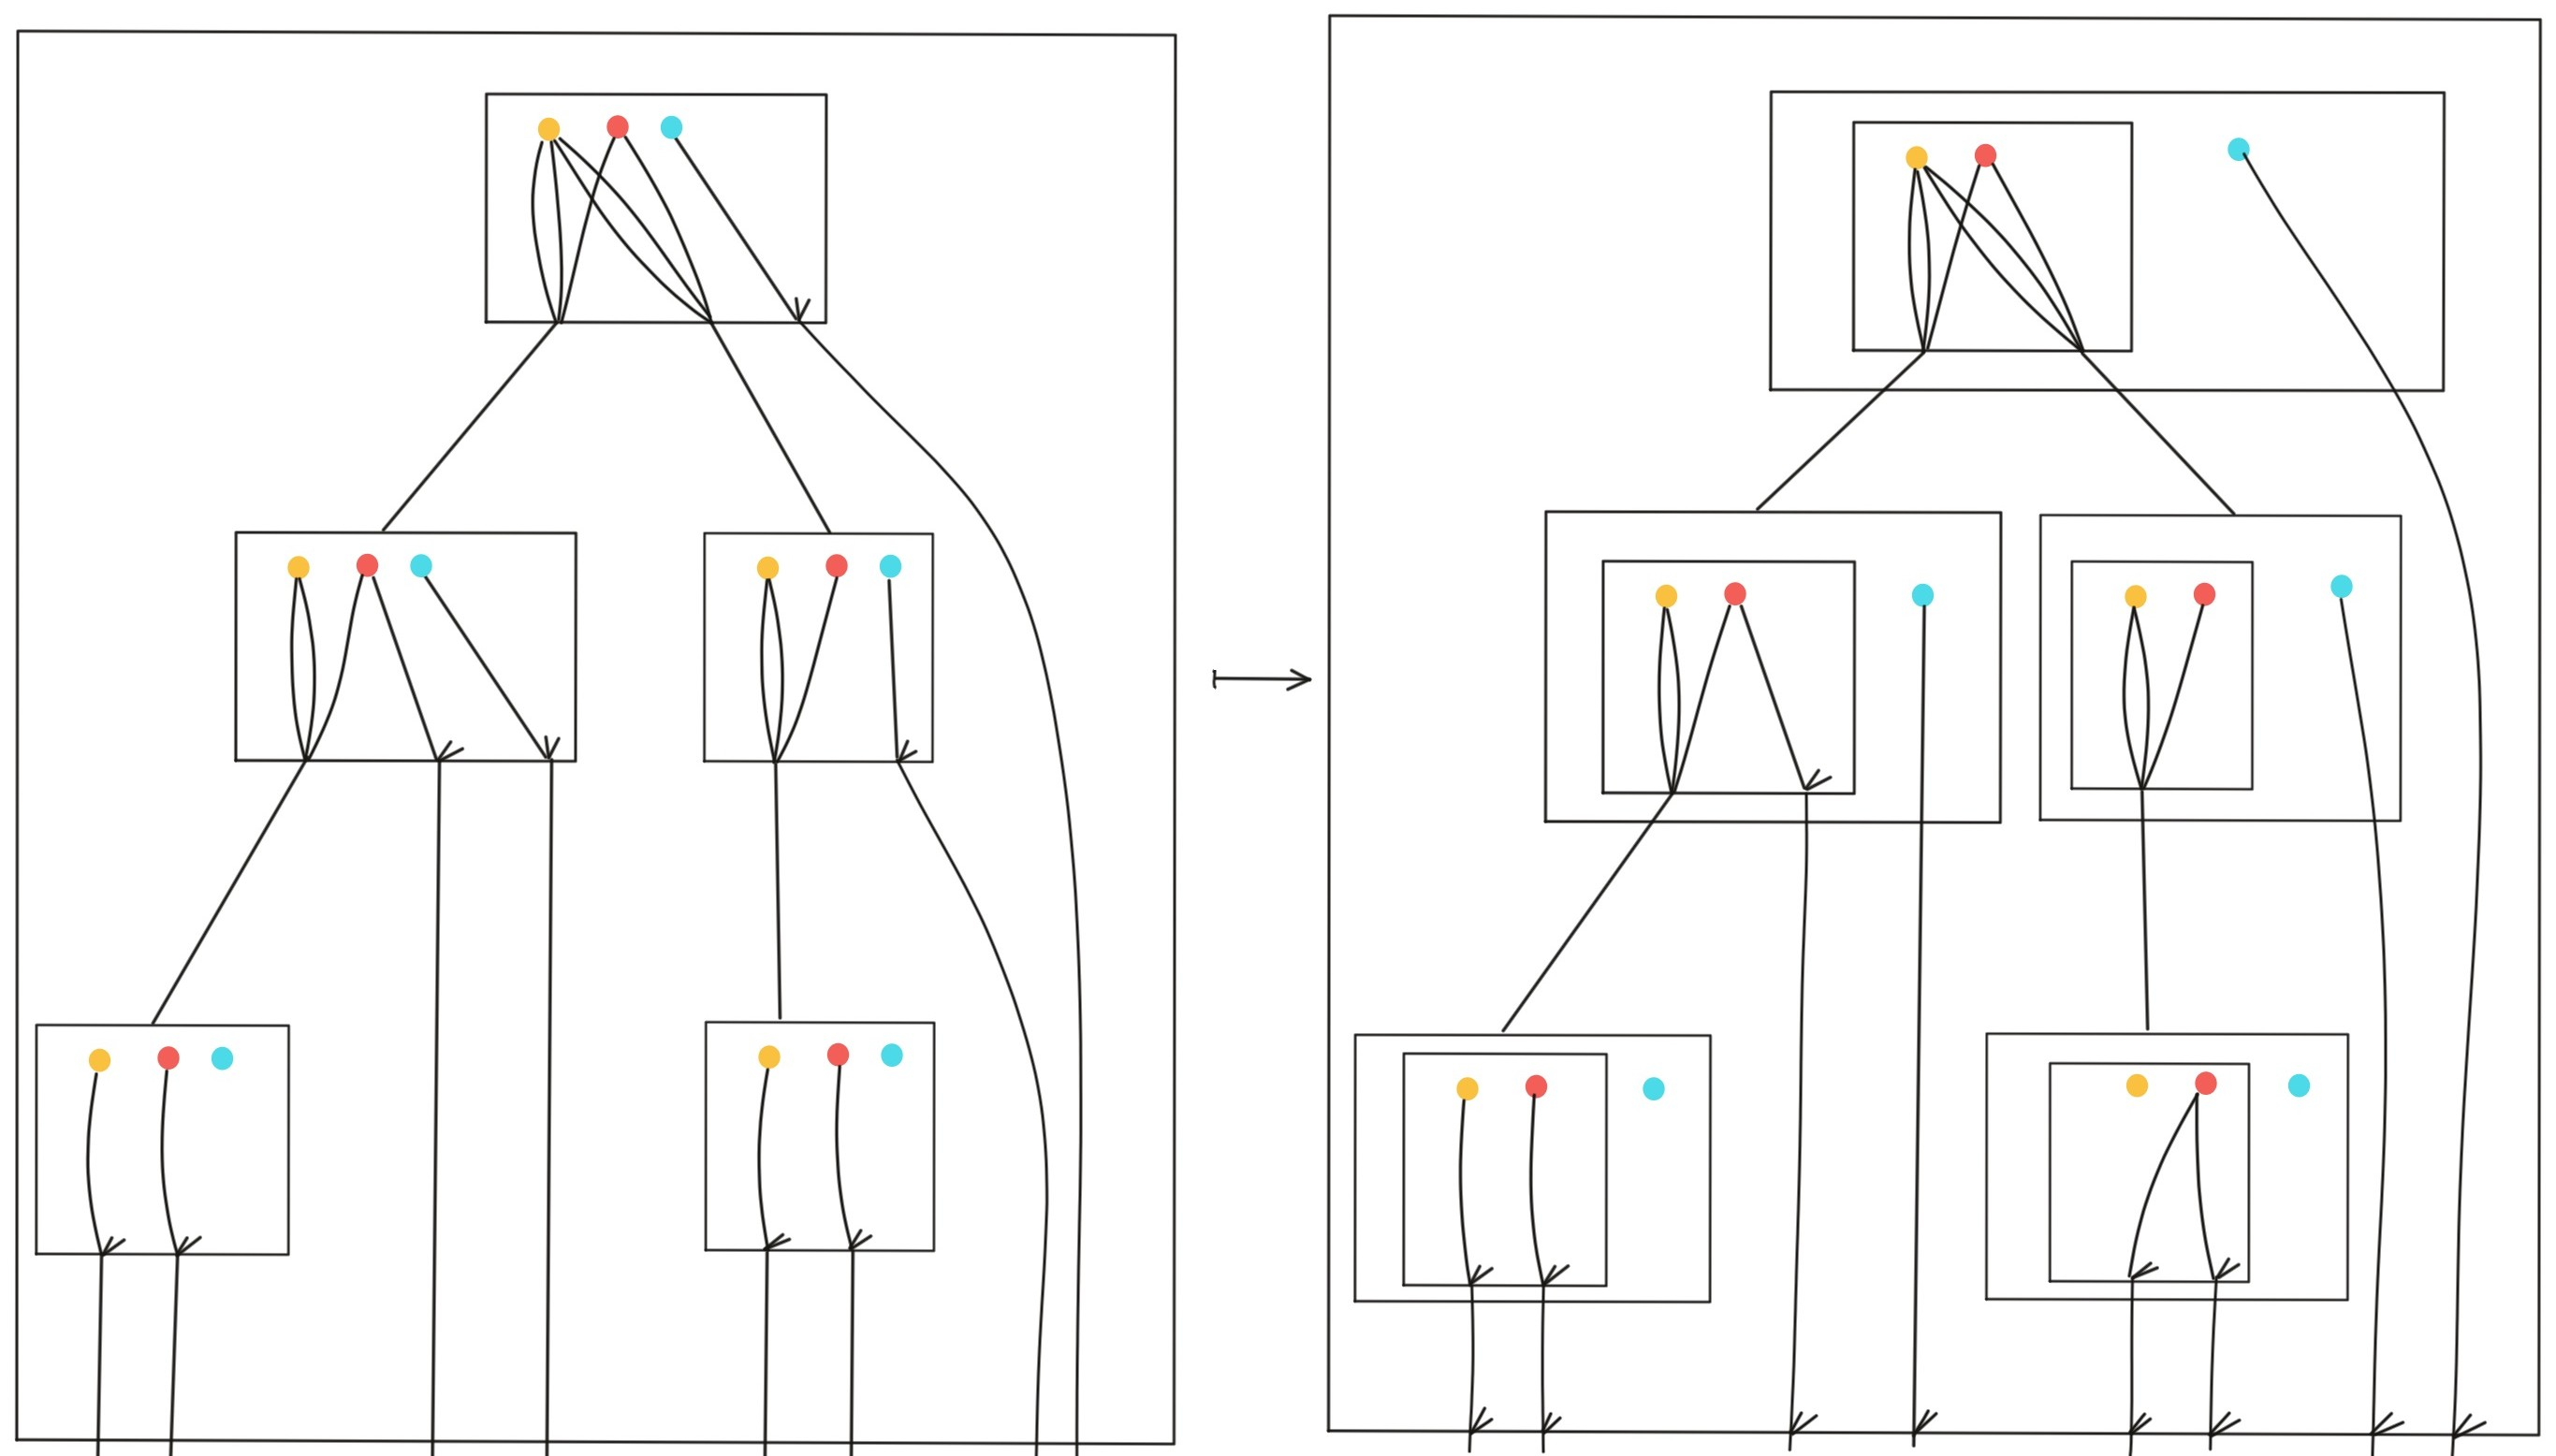
\includegraphics[scale=.1]{MyPic20.jpg}
\end{center}
\item After that, we lift to $\reduce k$ the function function
\begin{align*}
\ranked{\tmonad(\reduce k\Sigma^{k-1}\otimes \Sigma) \to \tmonad\mati {k-1} {(\Sigma\cdot(1+\Sigma))}\otimes \Sigma}
\end{align*}
which pulls-up the last component of the tensor product to the parents, as illustrated by the following picture 
\begin{center}
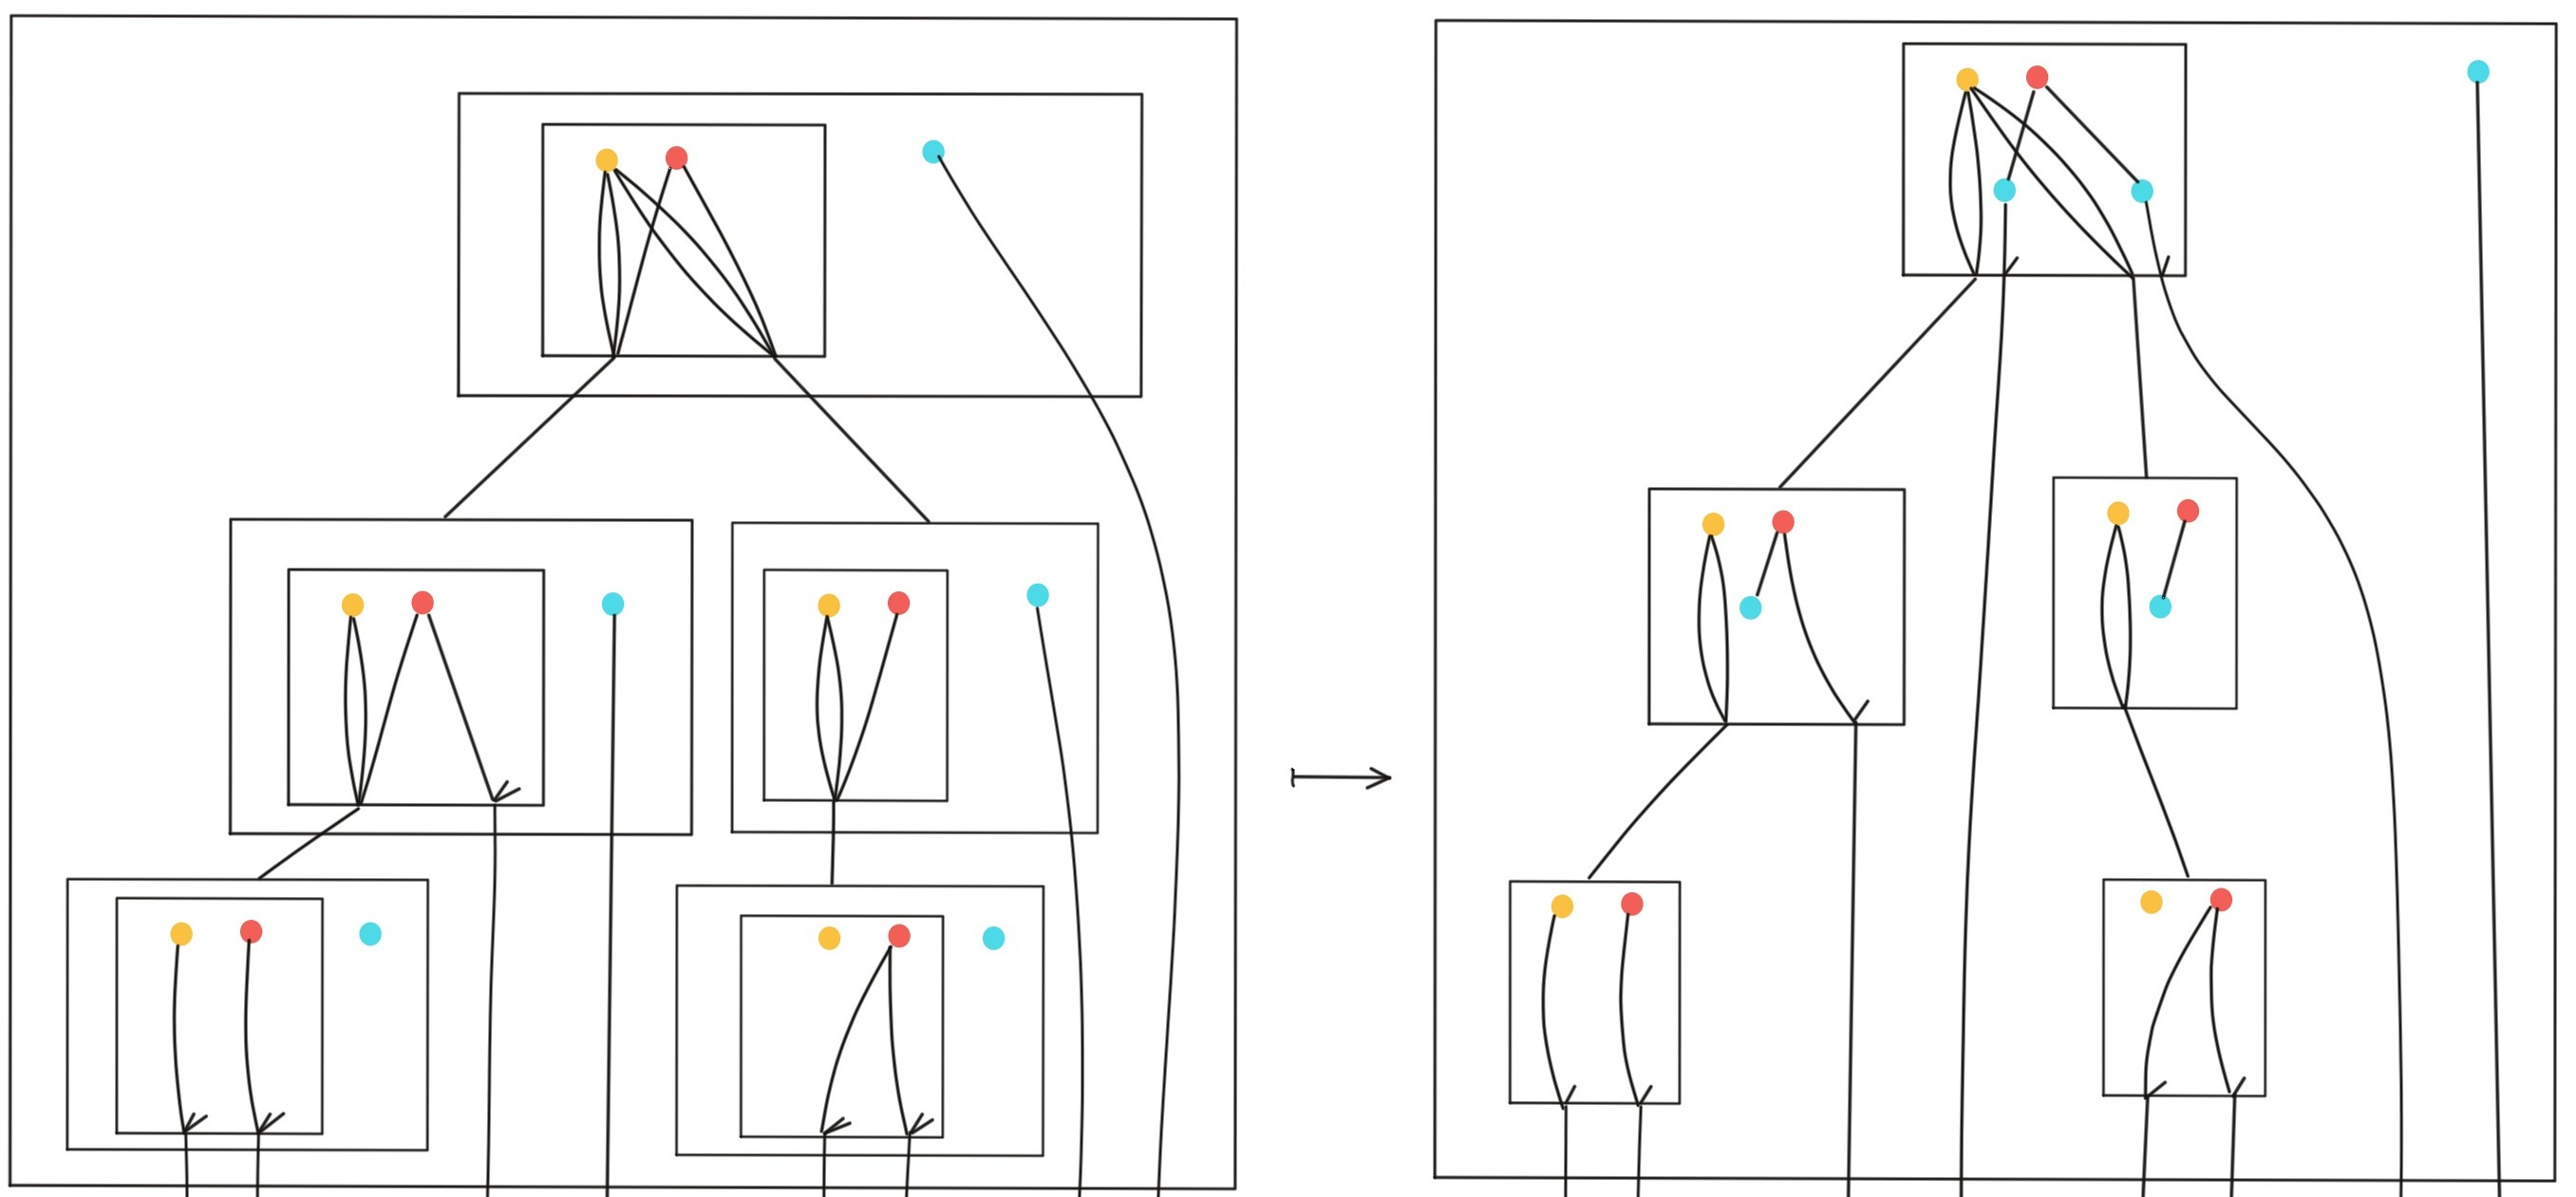
\includegraphics[scale=.12]{MyPic21.jpg}
\end{center}
\item After that, we apply the induction hypothesis to unfold the term from $\ranked{\tmonad\mati {k-1} {(\Sigma\cdot(1+\Sigma))}}$. Finally, after some operations aiming at adjusting the type of the output term, we get our result.
\end{enumerate}
Clearly, the most important steps are 1 and 2. We explain in the following how they can be derived. 

Consider the function 
\begin{align*}
\ranked{f:\tmonad \reduce k (\Gamma\otimes \Sigma)\to \reduce k \tmonad(\reduce k \Gamma\otimes \Sigma)}
\end{align*}
Obtained as follows. First we lift the basic function
\begin{align*}
\ranked { \reduce k (\Gamma\otimes \Sigma) \to  \reduce k (\reduce k \Gamma\otimes \Sigma)}
\end{align*}
to terms. Then we compose the result with the following function, obtained by composing the unfold function with the function of Example~\ref{}
\begin{align*}
 \ranked{\tmonad \reduce k (\reduce k \Gamma\otimes \Sigma) \xrightarrow{\text{Unfold}}
 \reduce k \tmonad (\reduce k \Gamma\otimes \Sigma)\cdot \tmonad \reduce k (\reduce k \Gamma\otimes \Sigma) \xrightarrow{\text{Ex}~\ref{}} \reduce k \tmonad (\reduce k \Gamma\otimes \Sigma)}
\end{align*}
The function of step 1 is the function $\ranked{f}$ where $\ranked{\Gamma}$ is taken to be $\ranked{\Sigma^{k-1}}$.



Now consider that the function
\begin{align*}
\ranked{g:\tmonad (\reduce k \Gamma \otimes \Sigma) \to \tmonad \reduce {k-1} (\Gamma\cdot(1+\Sigma))\otimes \Sigma}
\end{align*}
which, for every node (describe). Here is an example illustrating the effect of the function $\ranked{g}$ on the term $t$ below which will be our running example in this proof.
\begin{center}
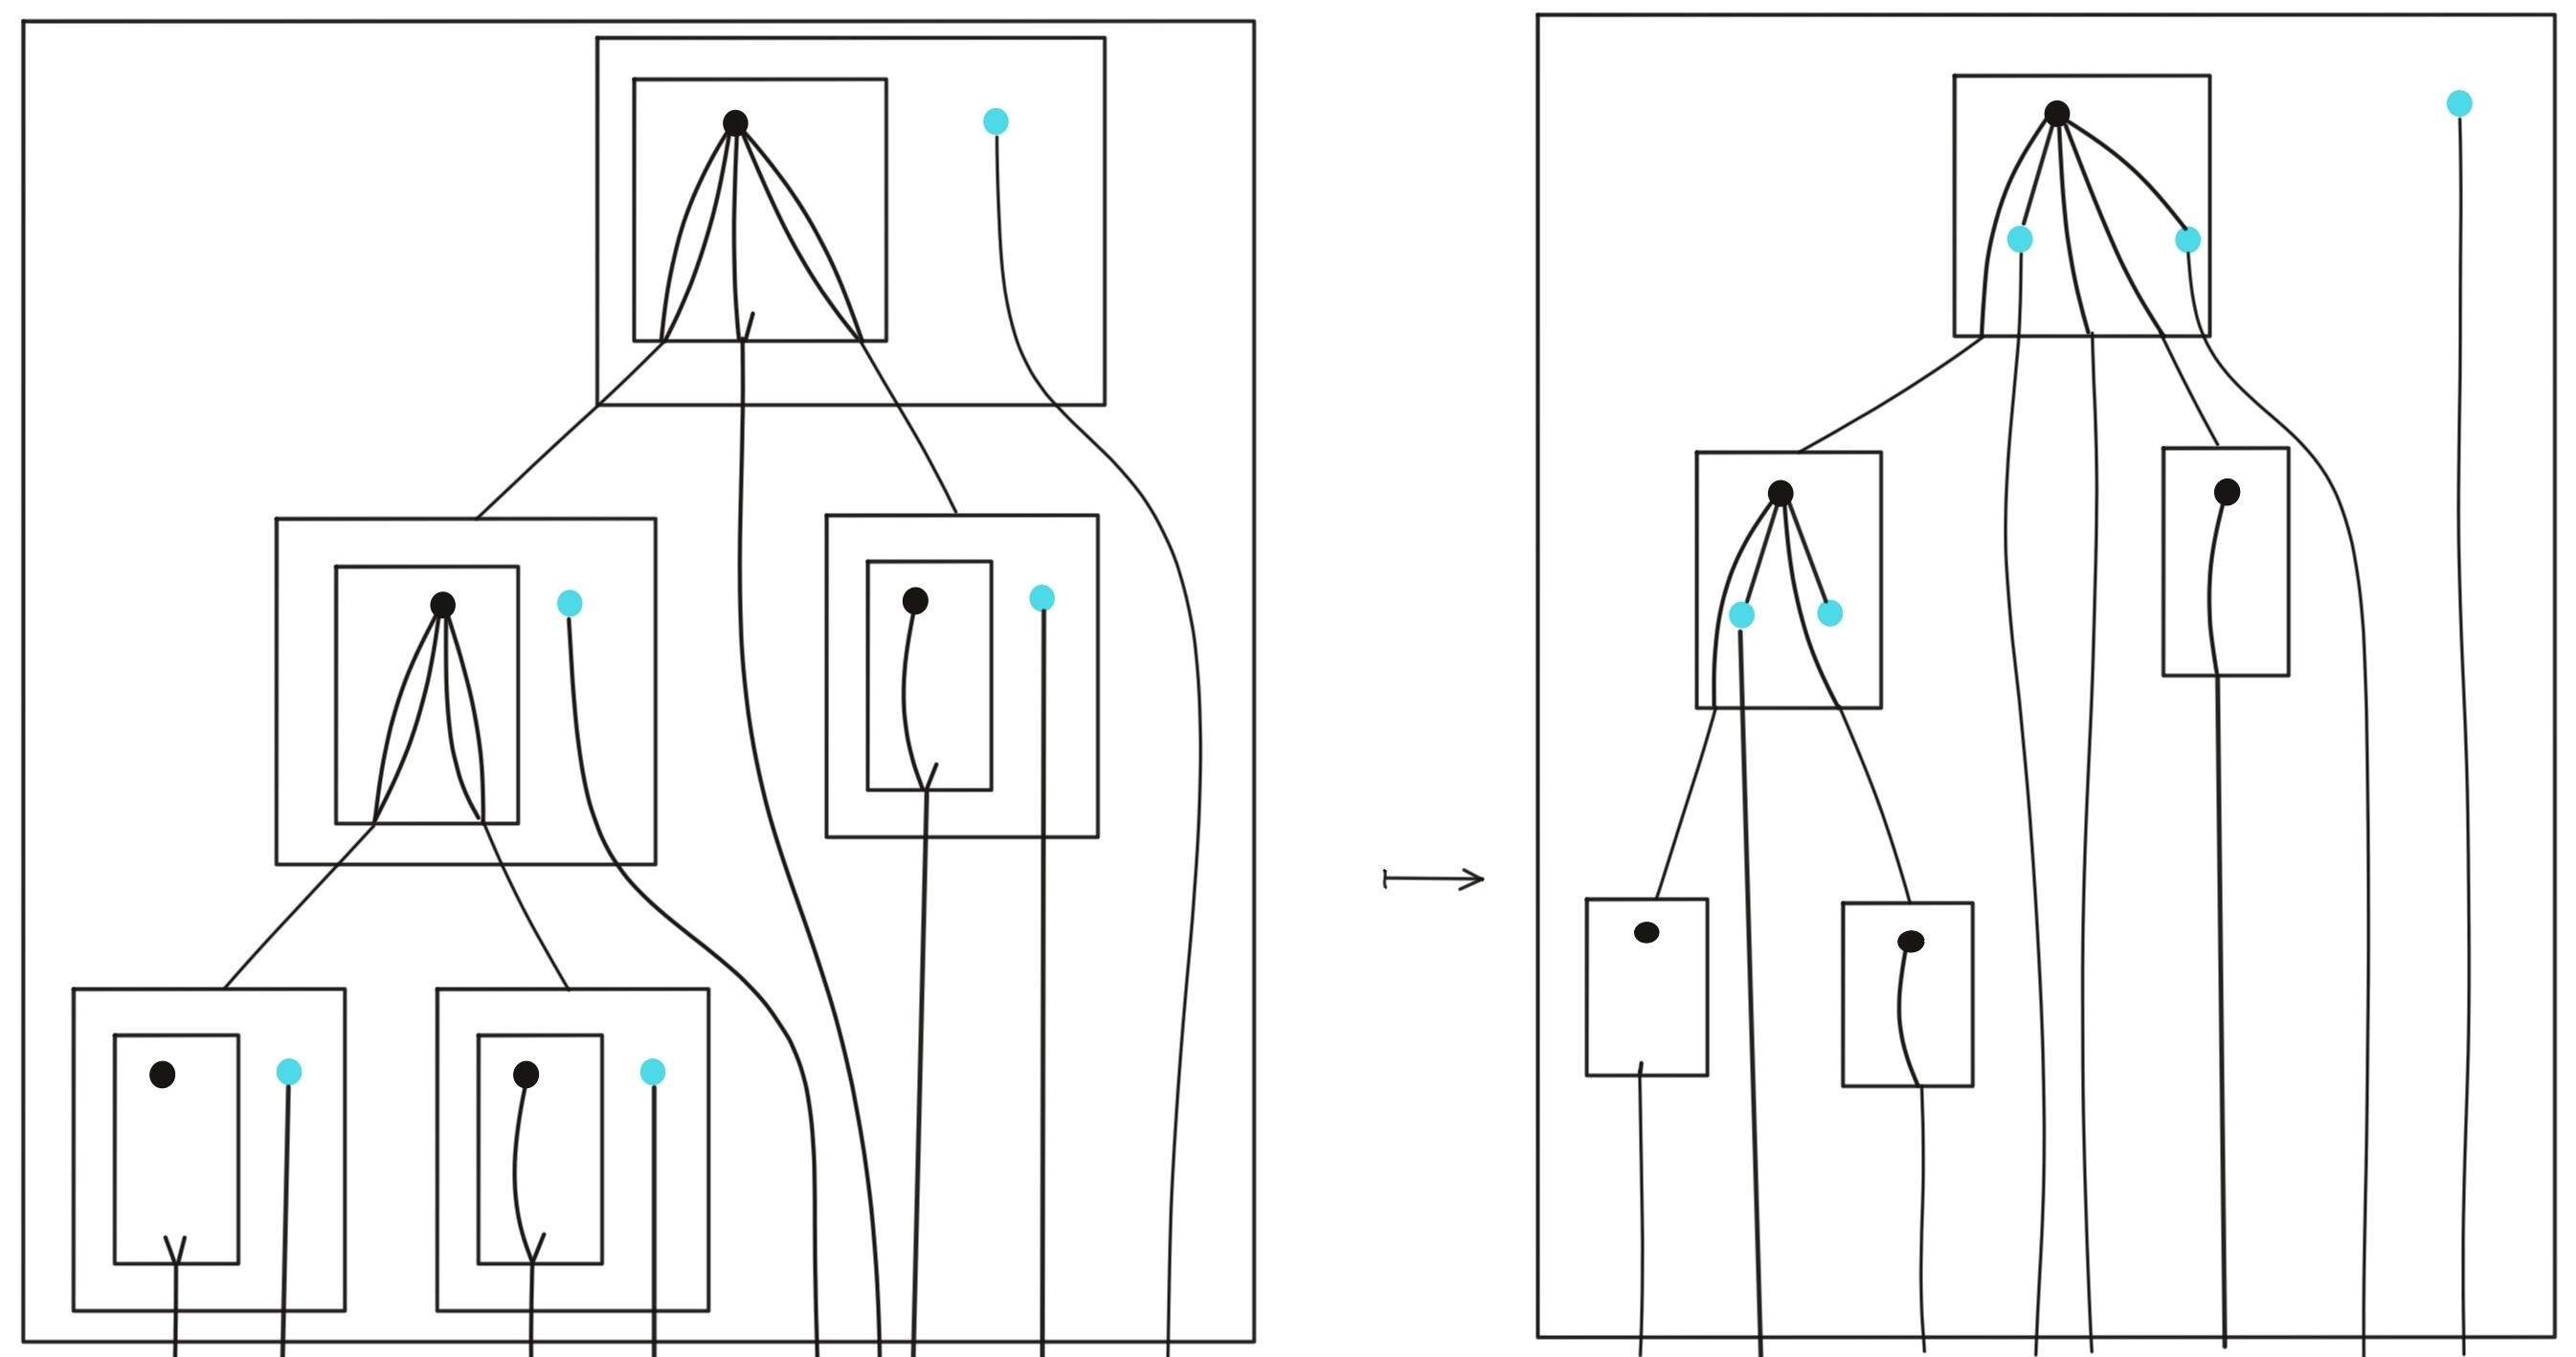
\includegraphics[scale=.12]{MyPic22.jpg}
\end{center}
The function of step 2 is obtained by taking $\ranked{\Gamma}$ to be $\ranked{\Sigma^{k-1}}$ in $\ranked{g}$. Let us see how $\ranked{g}$ can be derived.

First, we embed the tensor product into terms using the derivable function
\begin{align*}
\ranked{\reduce k \Gamma \otimes \Sigma \to \tmonad (2+\reduce k \Gamma +\Sigma)}
\end{align*}
After lifting this function to terms, and flattening the result, we get a term in $\ranked{\tmonad(2+\reduce k \Gamma +\Sigma)}$. 
Consider now the factorisation of these terms
 which is descibed as follows. There is two types of factors
\begin{itemize}
\item  A factor of the first kind is of depth at most three. Its root is a $\reduce k \rGamma$ element, it contains the children of the root labeled by $2$ and the grand-children labeled by elments from $\rSigma$.
\item If a node is labeled by $2$ or by an element of $\rSigma$, and it is not part of a factor of the first kind, then it forms a singleton factor of its own.    
\end{itemize}
This factorisation is of type
\begin{align*}
\ranked{\tmonad(2+\reduce k \Gamma +\Sigma) \to \tmonad(\reduce k \Gamma\cdot(1+2)\cdot(1+\Sigma)+\tmonad(2+\Sigma+\reduce k \Gamma))}
\end{align*}
Where the type of the first kind of factors is $\ranked{\reduce k \Gamma\cdot(1+2)\cdot(1+\Sigma)}$, the elment $1$ is used when a child of the root is not $2$ or a grand child is not an element of $\rSigma$. 
This factrorisation can clearly be implemented by a first-order rational function. After these operations, our example term $t$ becomes like this, where the binary gray node is the element $2$, we ommited the element $1$ in the figure, and the factorisation is indicated by the red lines
\begin{center}
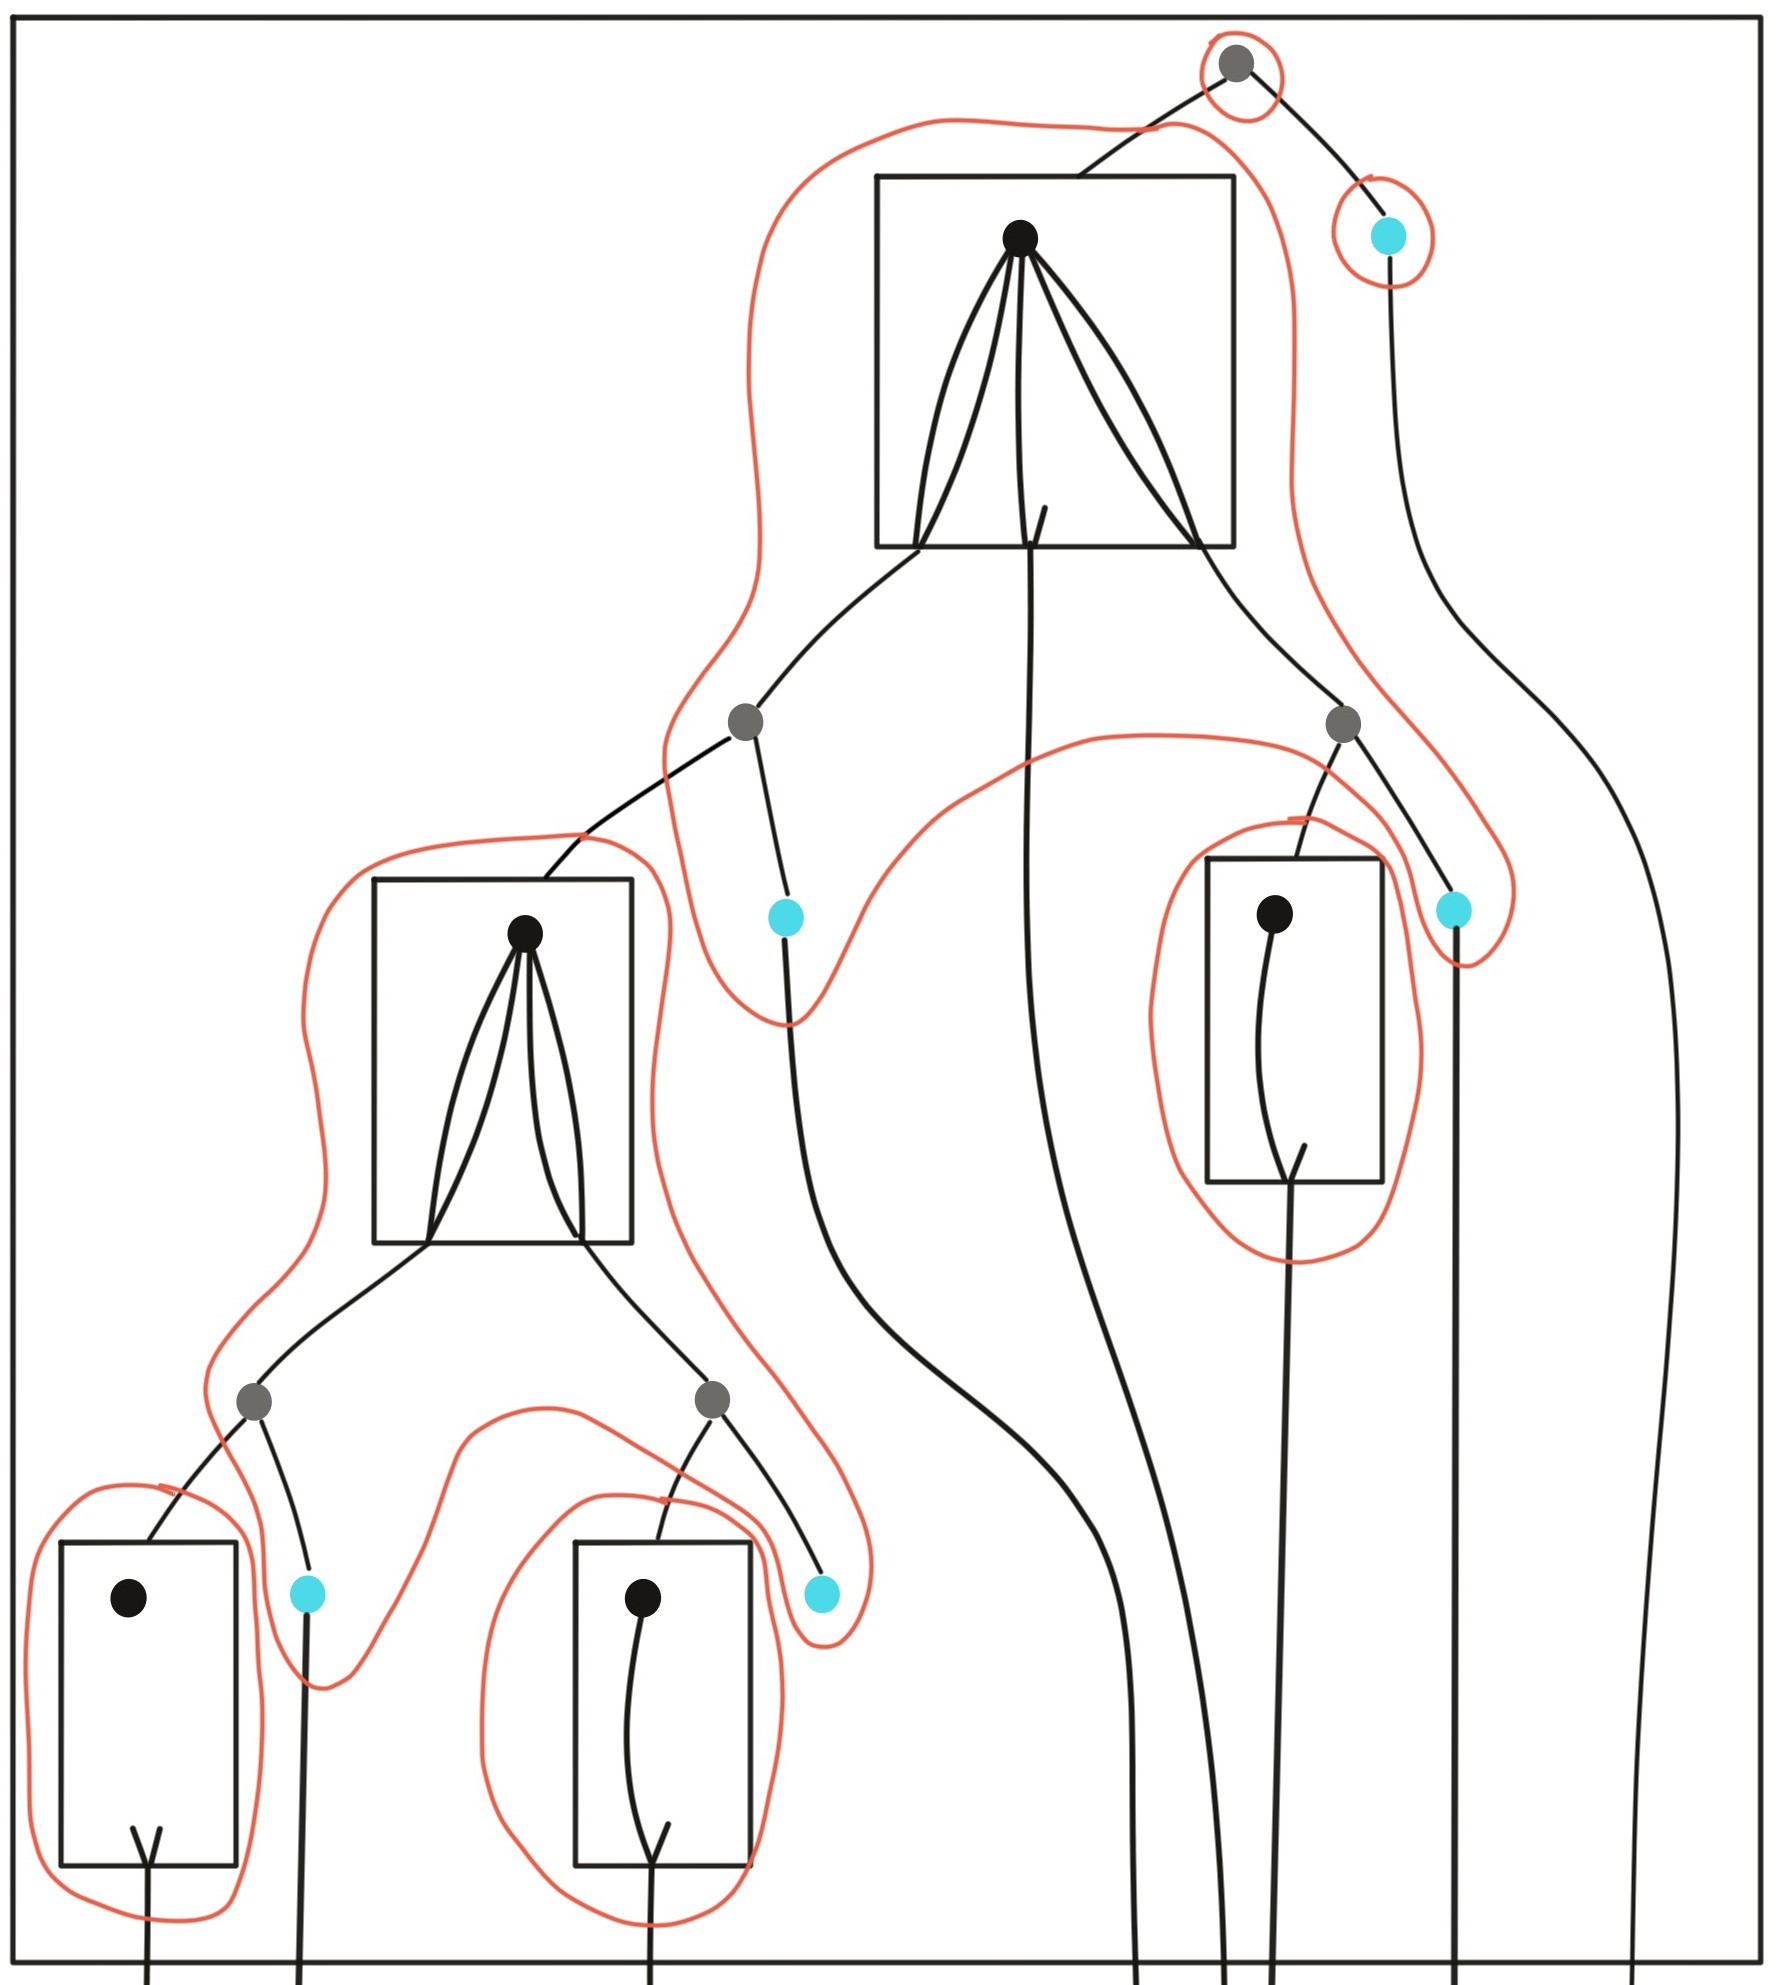
\includegraphics[scale=.1]{MyPic23.jpg}
\end{center}
  After that, we apply to each block of the first kind the homomorphism that transforms every element $2$ into the following element of type $\ranked{\mati k 1}$
  \begin{center}
  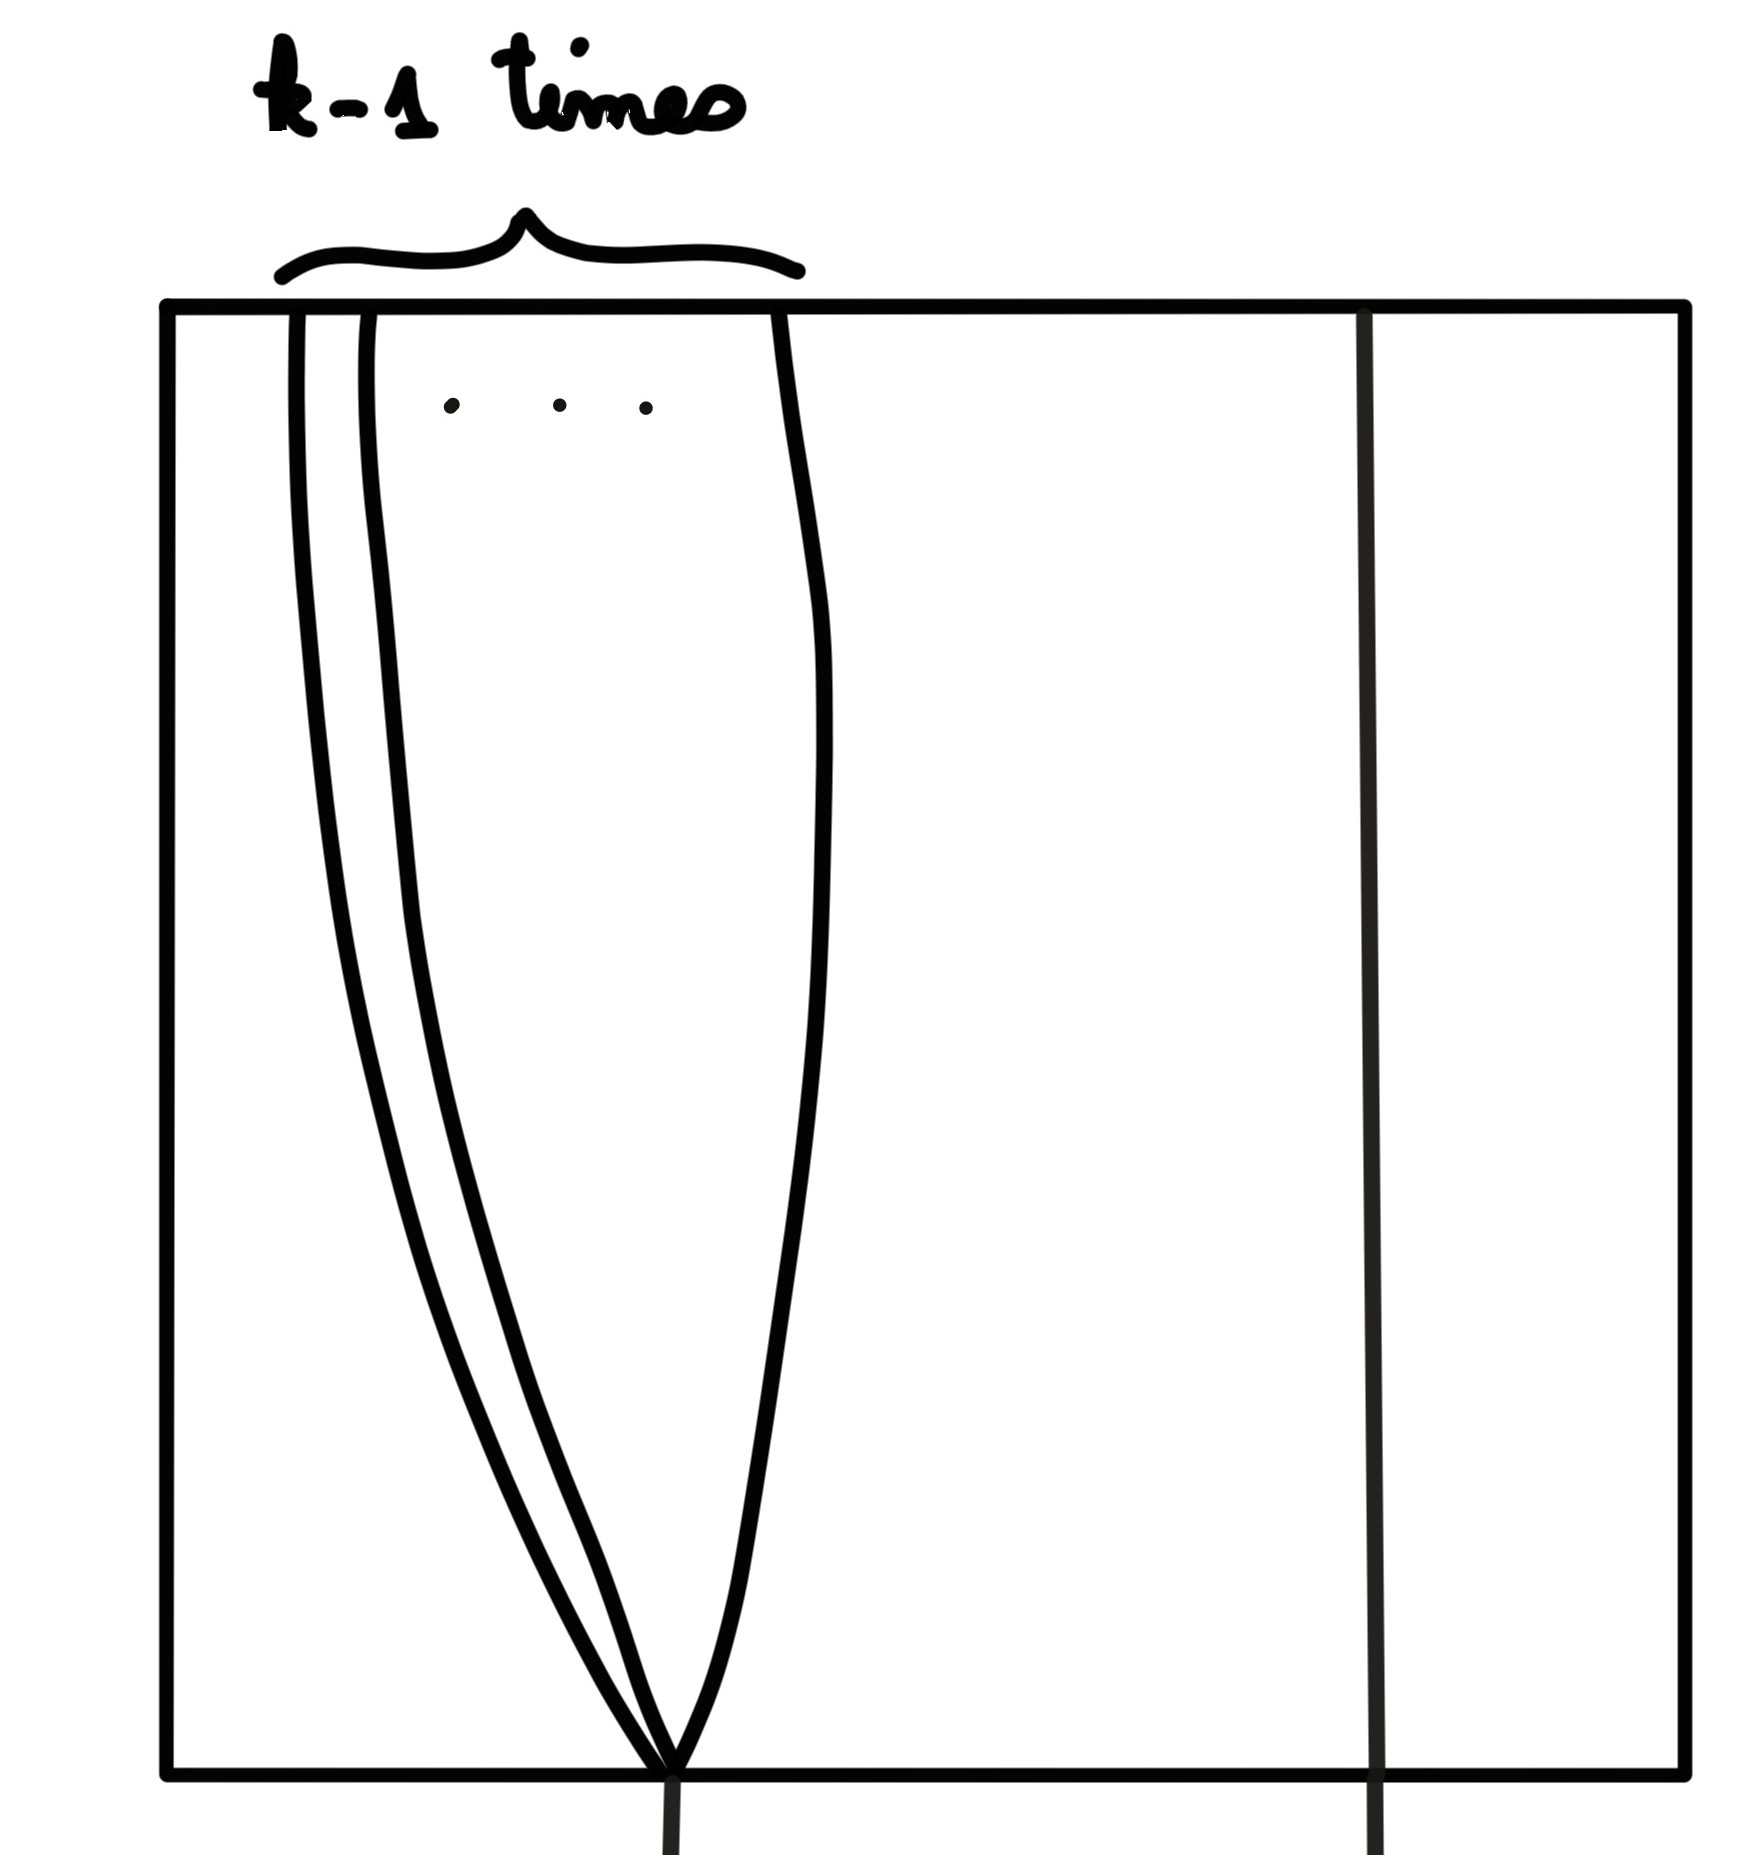
\includegraphics[scale=.05]{MyPic24.jpg}
  \end{center}
  and keeps the other nodes unchanged. The term $t$ becomes now
  \begin{center}
  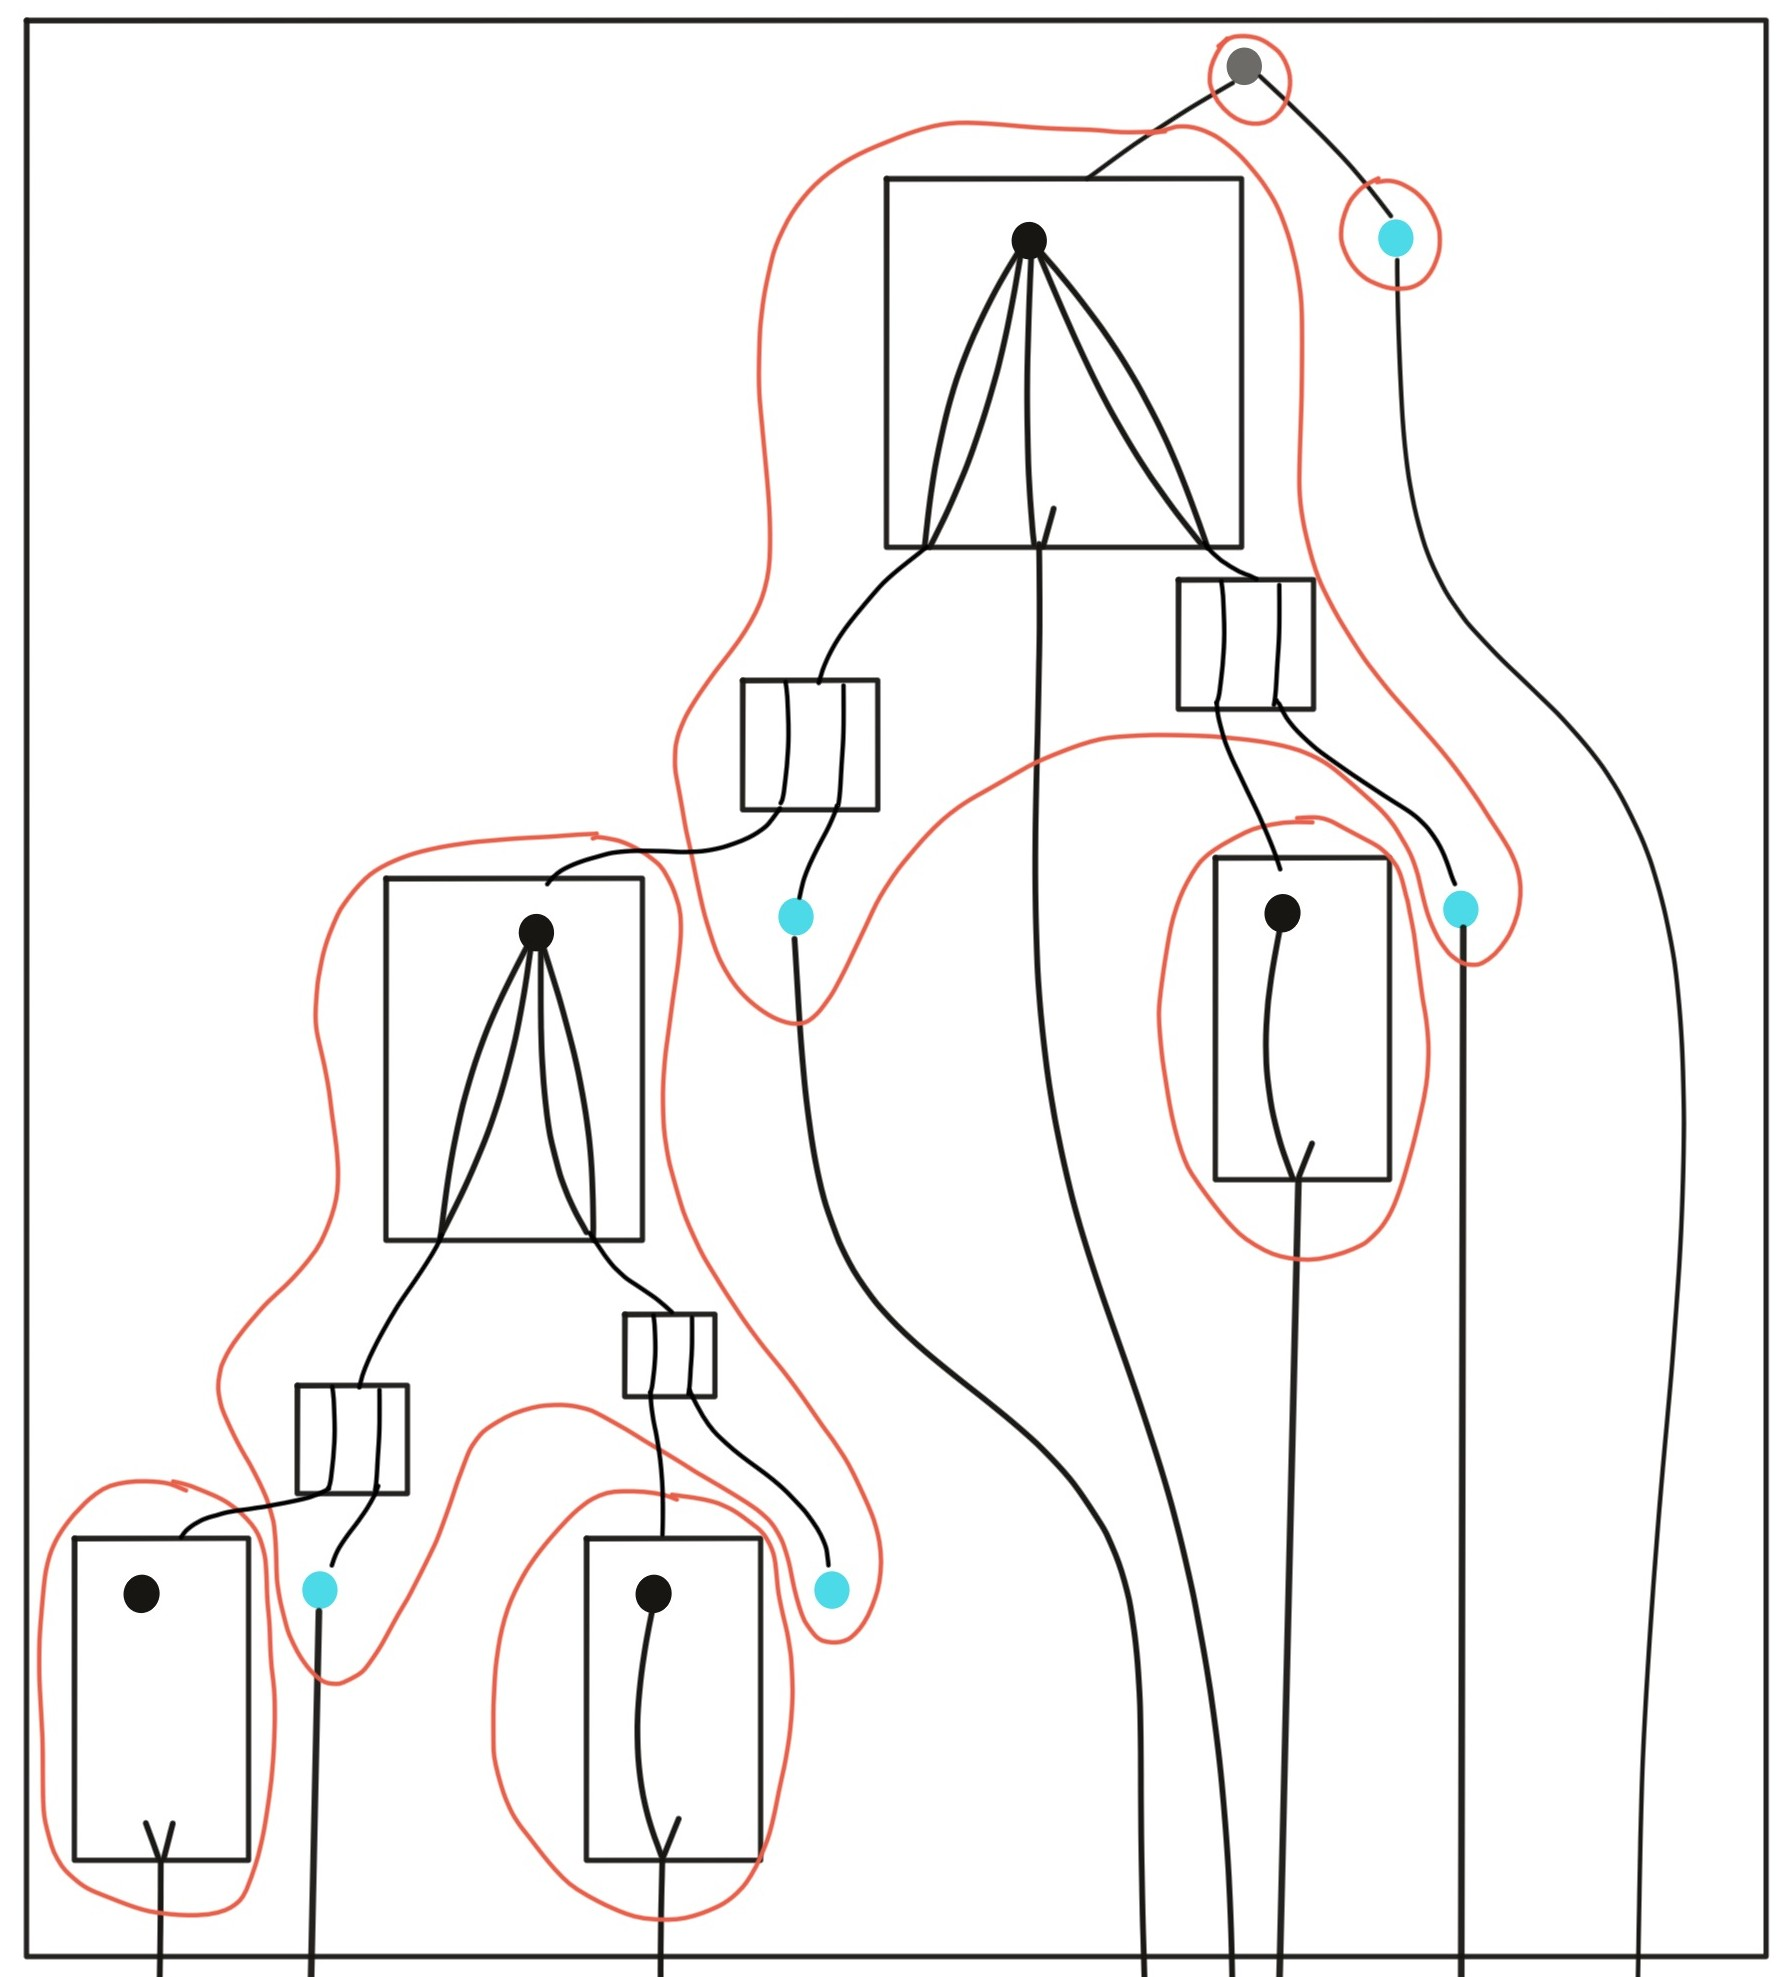
\includegraphics[scale=.1]{MyPic25.jpg}
  \end{center}
  We can now lift the partial shallow unfold (Example~\ref{}), followed by an injection and the elimination of $1$ to recover the type $\ranked{\reduce k \Gamma}$
  \begin{align*}
  \ranked{\reduce k \Gamma\cdot(1+\mati k 1)\to \reduce k (\Gamma\cdot(1+1))\to \reduce k (\Gamma\cdot 1) \to  \reduce k \Gamma}
\end{align*}
which result into a term of type $\ranked{\tmonad(\reduce k\Gamma\cdot(1+\Sigma)+\tmonad(2+\Sigma+\reduce k \Gamma))}$. We apply then the following basic functions, which aims at putting the $\cdot$ inside the scope of $\reduce k$, then reducing the degree of the fold:
\begin{align*}
\ranked{\reduce k\Gamma\cdot(1+\Sigma)\to \reduce k(\Gamma\cdot(1+\Sigma))\to \reduce {k-1}(\Gamma\cdot(1+\Sigma)\cdot (0+1)) }
\end{align*}
After that, we apply some flattening to get the desired term. However, we still dont have the right type. I need either a bottom, or something else to handel the garbage.
\end{proof}

%We will show this lemma by induction on $k$. For that, we need to strengthen the invariant of the induction: we will show that the unfolding of $\alpha$-homogenous terms in $\ranked{\tmonad \reduce l\rSigma^k}$ is derivable. Note that Lemma~\ref{lem:homo-twist} is the particular case of this statement where $k=l$. To state this strengthening more precisely, we need to generalize the definition of unfolding and $\alpha$-homogenuity to $\ranked{\tmonad \reduce l\rSigma^k}$ terms.
%
%
%
%If $k, l\in \set{2,3,\dots}$ such that $k\leq l$, we can embed the elements of $\ranked{\reduce l \rSigma^k}$ in 
%$\ranked{\mati l {(\rSigma+\set{0})}}$ by adding $l-k$ copies of the nullary element $0$ to the tensor product, as illustrated below:
%\begin{center}
%
%\end{center}  
%Hence, we can talk about the twist of an element of $\ranked{\reduce l \Sigma^k}$, and we can embed every element of $\ranked{\tmonad \reduce l \Sigma^k}$  into $\ranked{\tmonad \mati l \Sigma}$.
%
%We define the unfolding of a term $t$ in $\ranked{\tmonad \reduce l \Sigma^k}$ as its unfolding when seen as an element of $\ranked{\tmonad \mati l \Sigma}$. Note that the unfolding of a element of $\ranked{\tmonad \reduce l \Sigma^k}$ is an element of $\ranked{\reduce l(\tmonad (\Sigma+\set{0}))^k}$.
%
%We will be interested in a particular case of terms: the \emph{coherent} ones. We say that a term $t\in \ranked{\tmonad \reduce l \Sigma^k}$ is \emph{coherent} if the twist of every internal branche of $t$ seen as an element of $\ranked{\tmonad \mati l \Sigma}$ has $\set{1,\ldots,k}$ as domain. Note that the unfolding of a coherent element of $\ranked{\tmonad \reduce l \Sigma^k}$ is an element of $\ranked{\reduce l(\tmonad \Sigma)^k}$.
%
%
%For a monotone function 
%\begin{align*}
%\alpha: \set{1,\ldots,k} \to \set{1,\ldots,k}
%\end{align*}
%we say that a term $ t \in\ranked{\tmonad\reduce l \Sigma^k}$ is $\alpha$-homogeneous if  it is coherent and if all internal branches have as twist the function $\beta$ such that
%\begin{align*}
%\beta|_{\set{1,\dots,k}}=\alpha.
%\end{align*}
%Now we are ready to state the generalisation of our lemma.
%\begin{lemma}
% Let $k, l \in \set{1,2,\ldots}$ and let $\alpha : \set{1,\ldots,k} \to \set{1,\ldots,k}$ be a monotone function. There is a  derivable operation 
%    \begin{align*}
%        \ranked{f : \tmonad \reduce l \rSigma^k \to \reduce {l} {(\tmonad \Sigma)}^k }
%        \end{align*}      
%which coincides with term unfolding for all inputs which are $\alpha$-homogeneous.
%\end{lemma}
%As said earlier, we proceed by induction on $k$. When $k=1$, unfolding coincides with the basic function
%\begin{align*}
%\ranked{\mathsf{unfold} : \tmonad \reduce l \rSigma \to \shallowterm{\reduce {l} {\tmonad \Sigma}} {\tmonad \reduce l \rSigma}  }
%\end{align*}
%We only need to adjust the output type, that is to get rid of the $\ranked{\tmonad \reduce l \rSigma}$ after the ``$\cdot$'' of the shallow term. Fisrt, we lift the basic function 
%\begin{align*}
%\ranked{\composeterm: \tmonad \reduce l \rSigma \to 
%        1 + \shallowterm {\reduce l \rSigma} {\tmonad \reduce l \rSigma}}          
%\end{align*} 
%and the identity function 
%\begin{align*}
%\ranked{ \reduce {l} {\tmonad \Sigma}\to \reduce {l} {\tmonad \Sigma}}          
%\end{align*} 
%to the the shallow combinator. \todo{Je ne sais pas comment finir.}
